\begin{figure}[t]

    \centering
	\renewcommand{\arraystretch}{0.8}
    
    \begin{tabular}{|c c c c c|}
    	
		\hline

		(a) & (b) & (c) & (d) & (e) \\
		
		\hline
		{} & {} & {} & {} & {} \\
		
		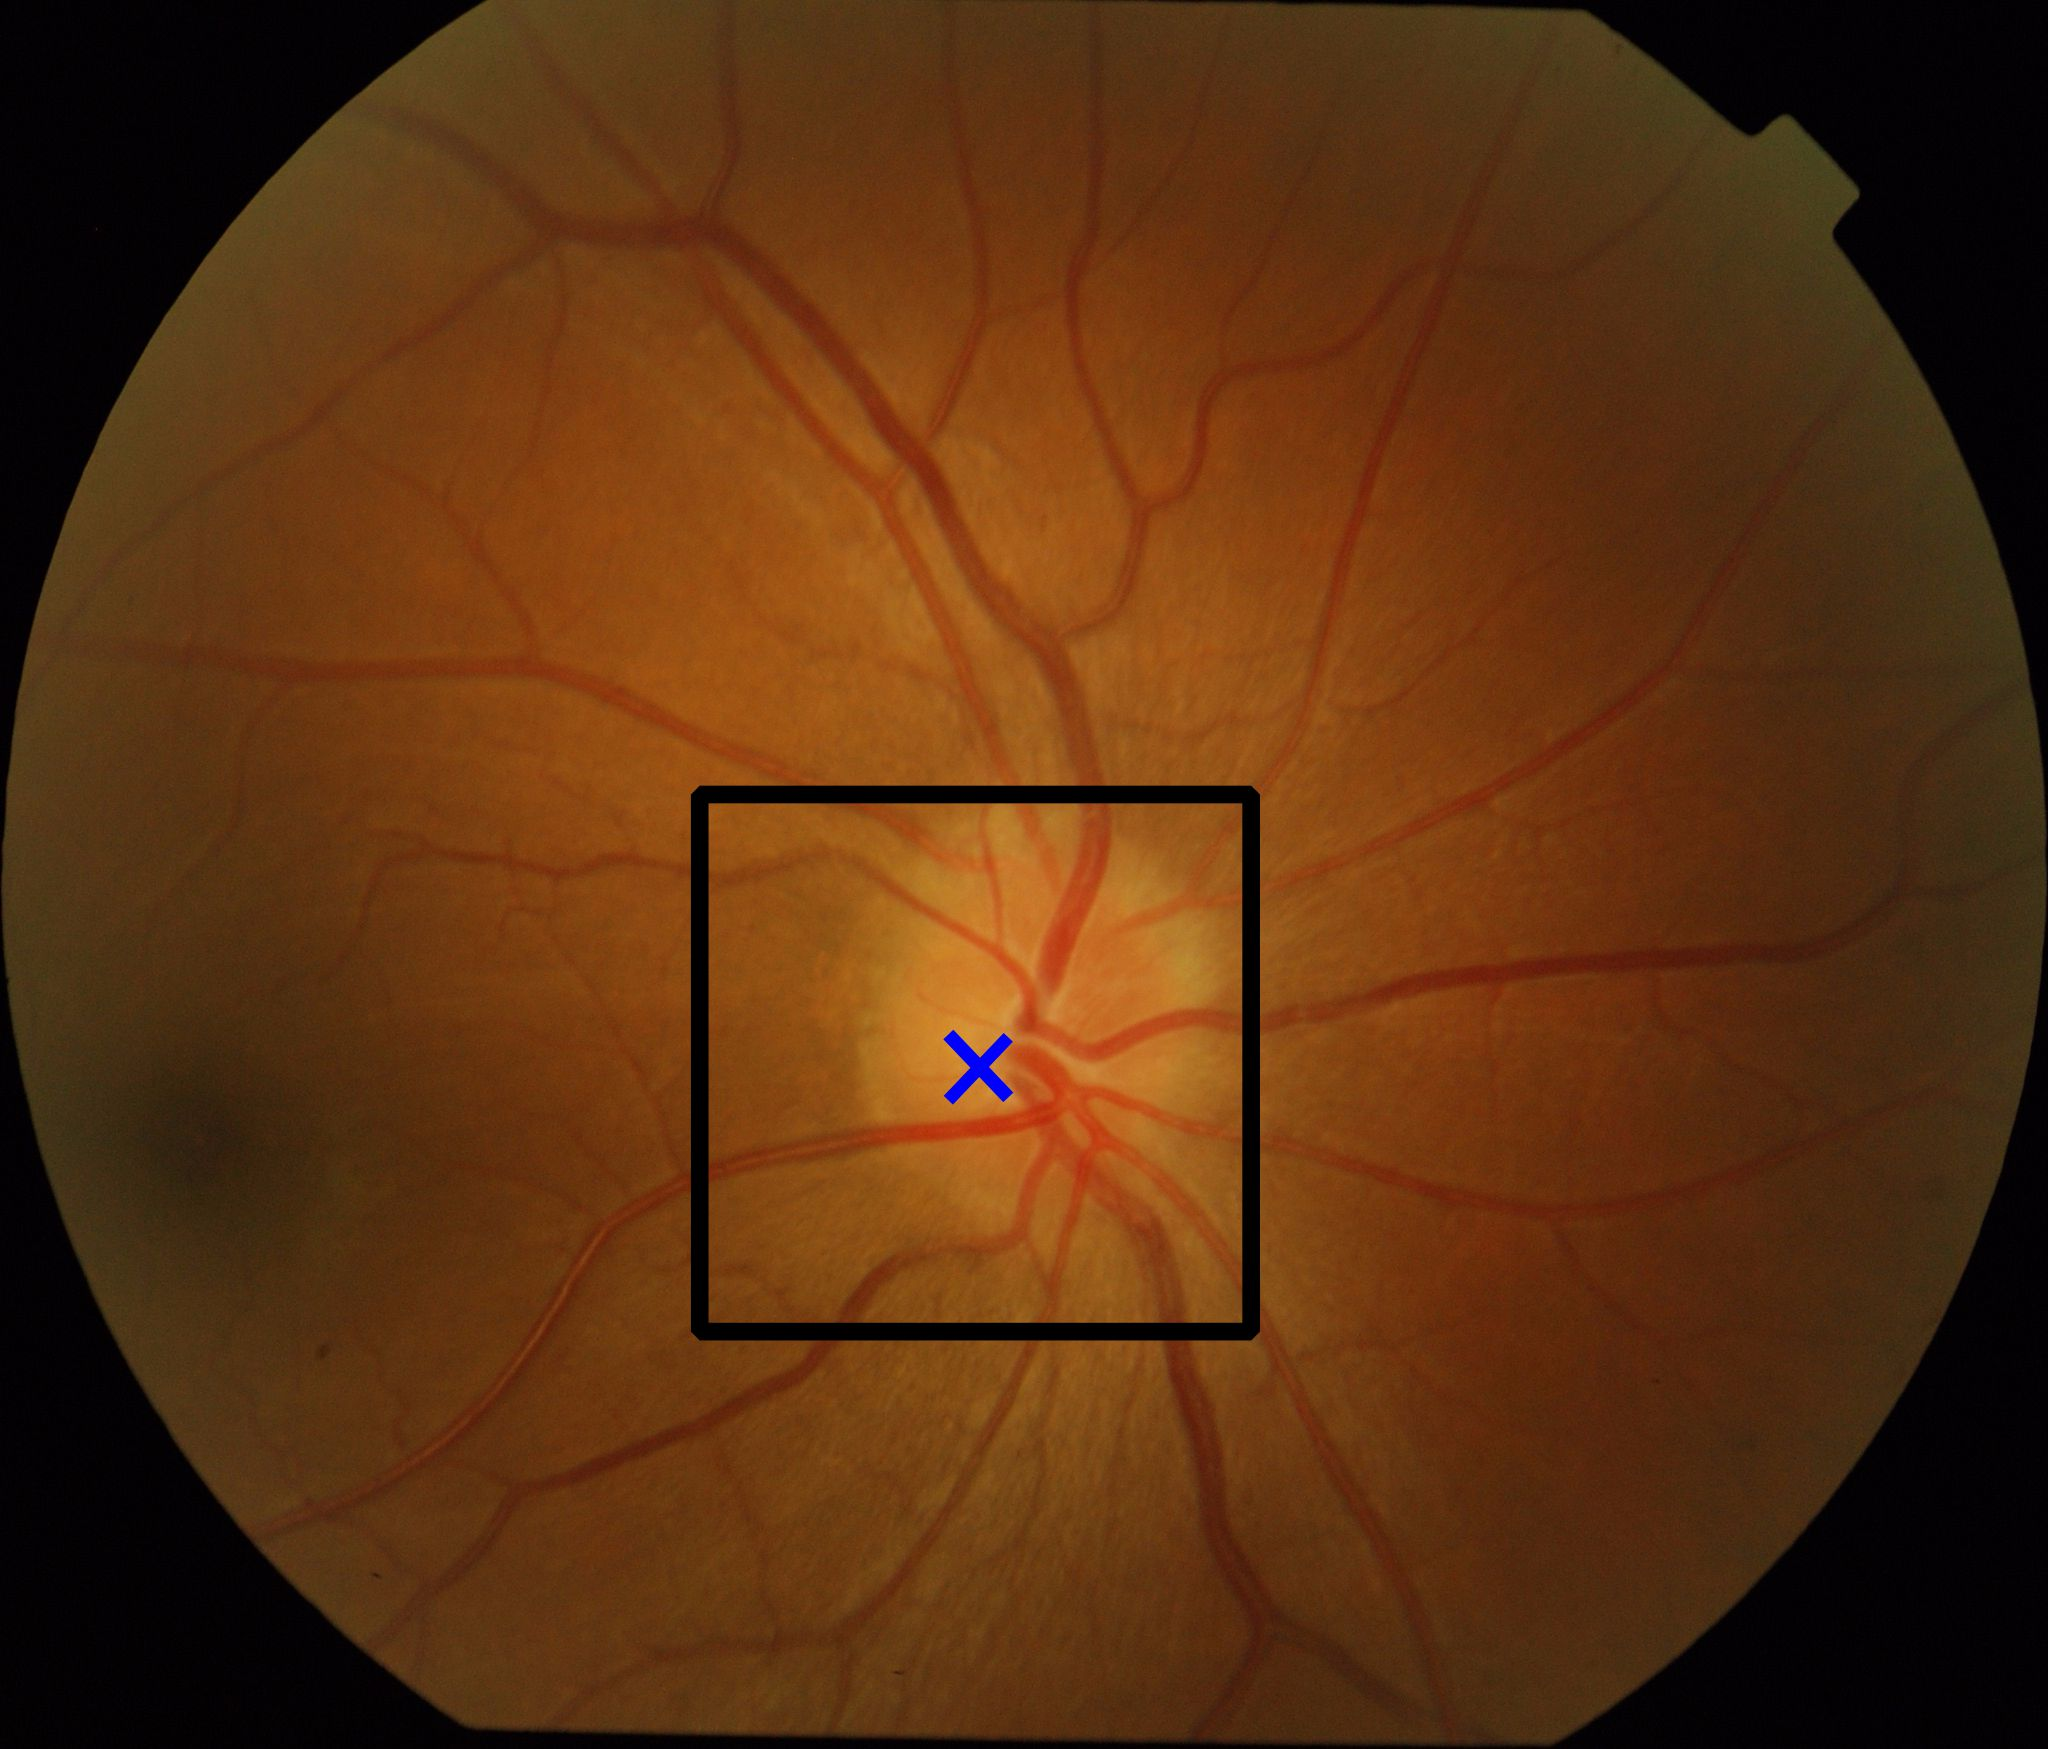
\includegraphics[width=3.5cm]{Images/Results/Segmentation/drishti101/od_detect.jpg} &
		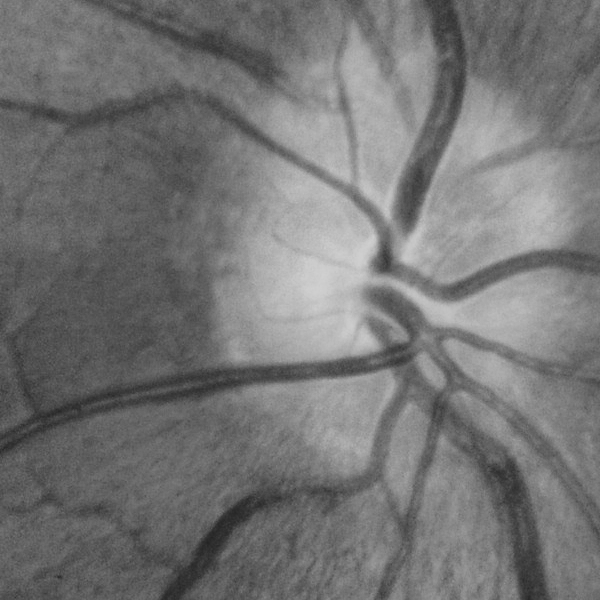
\includegraphics[width=3cm]{Images/Results/Segmentation/drishti101/0_crop.png} &
		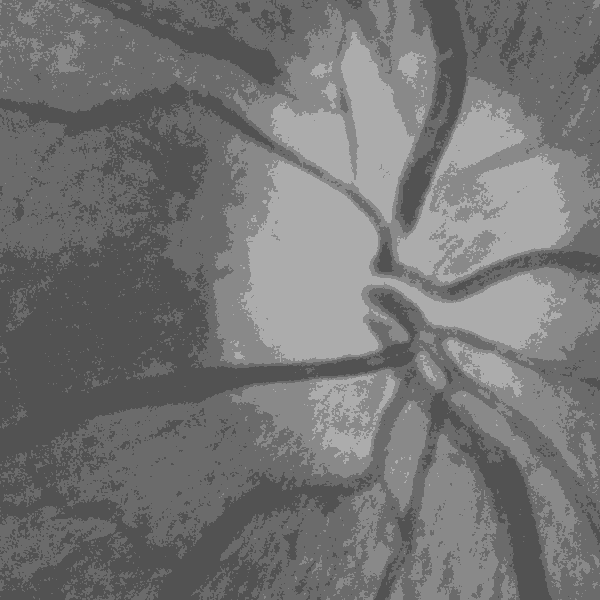
\includegraphics[width=3cm]{Images/Results/Segmentation/drishti101/1_kmeans.png} &
		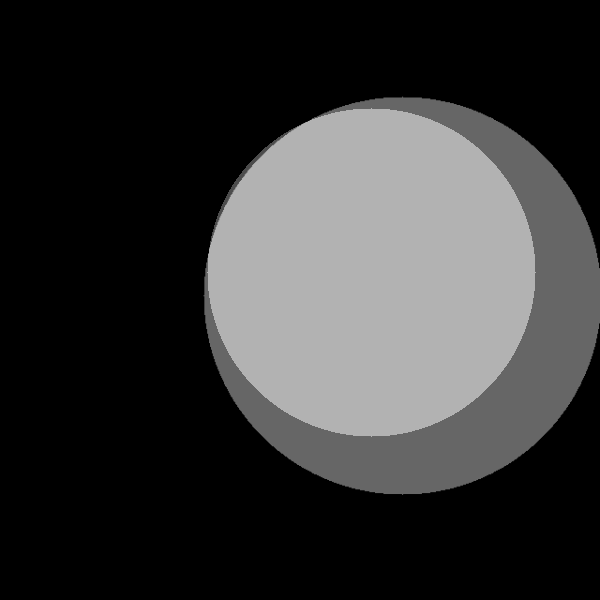
\includegraphics[width=3cm]{Images/Results/Segmentation/drishti101/overlay.png} &
		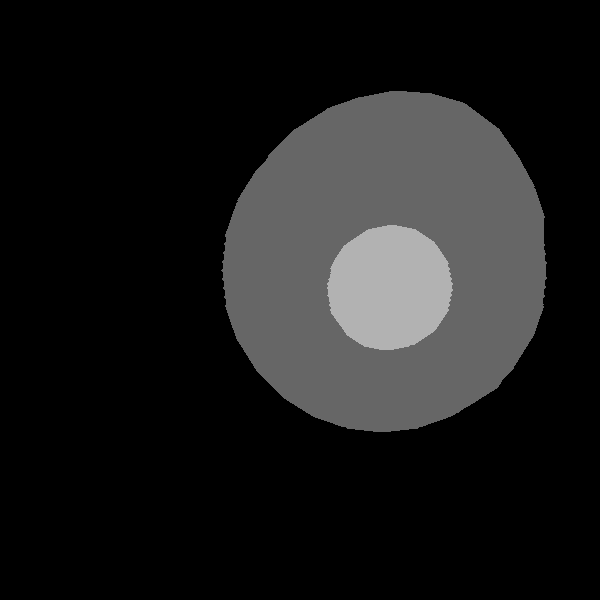
\includegraphics[width=3cm]{Images/Results/Segmentation/drishti101/overlay_gt.png} \\
		
		{} & {} & {} & CDR = 0.67 & CDR = 0.16 \\
		{} & {} & {} & $\updownarrow$ & $\updownarrow$ \\
		{} & {} & {} & Glaucomatous & Healthy \\
		
		\hline
    
    \end{tabular}

	\caption{\label{glaucoma_screening_failures}Glaucoma screening failure: (a) original retinal image, with OD location point (b) ROI extraction: sub-image around the OD, (c) k-means clustering (K=4), (d) joint OC-OD segmentation with CDR result and final diagnosis, (e) ground-truth joint OC-OD segmentation with CDR result and final diagnosis. The resulting segmentation leads to overestimated regions, and the CDR computation conducts to a false positive prediction.}

\end{figure}

